In this and next chapter, we will focus on ``scalability bugs'', a new class of
bugs that was born in an era of cloud computing.  \xxx{talk about scale bugs}

This chapter highlights an urgency in tackling scalability bugs by studying
deeply in \totAll scalability bugs from different popular scalable distributed
systems. Section \ref{sec-scb-mot} discusses motivation in tackling scalability bugs
and Section \ref{mot-observe} gives some observations we gain from the study.

\section{Motivation}
\label{sec-scb-mot}

% scale, scale ... 
Is scale a friend or a foe \cite{Ousterhout+11-ScaleFriendEnemy}?
% CACM, is scale friend or enemy, john ousterhout
On the positive side, scale surpasses the limit of a single machine in
meeting users' increasing demands of compute and storage, which led to
many inventions of ``cloud-scale'' distributed systems
\cite{Chang+06-BigTable, 
DeanGhemawat04-MapReduce, 
DeCandia+07-Dynamo,
Ghemawat+03-GoogleFS, 
Hindman+11-Mesos,
Verma+15-Borg}.  The field has witnessed a
phenomenal deployment scale of such systems;
%
Netflix runs tens of 500-node Cassandra clusters \cite{RunningNetflix13},
% Running Netflix on Cassandra in the Cloud (youtube), Adriak Crockcroft
% https://www.youtube.com/watch?v=97VBdgIgcCU
Apple deploys a total of 100,000 Cassandra nodes \cite{WikiCassandra}, 
% https://en.wikipedia.org/wiki/Apache_Cassandra
and Yahoo! recently revealed the use of 40,000 Hadoop servers,
with a 4500-node cluster as the largest one \cite{LargestHadoop}.
% Http://www.techrepublic.com/article/why-the-worlds-largest-hadoop-installation-may-soon-become-the-norm/

% dark side, foe
On the negative side, scale creates new development and deployment issues.
Developers must ensure that their algorithms and protocol designs
to be scalable.
However, until real deployment takes place, unexpected bugs 
in the actual implementations are unforeseen.
% more and more
This new era of cloud-scale distributed systems has given birth
to a new type of bug: {\em scalability bugs}.  They are latent bugs that
are scale-dependent; they only surface in large-scale deployments, but not
in small/medium-scale ones.  Their presence jeopardizes systems
reliability and availability at scale.

As an example, let us consider a bug in Cassandra, a
highly-scalable peer-to-peer key-value store.  If a customer initially
deploys a cluster of 50 nodes and later scales it out with 50 additional
nodes, the operation can be done smoothly.  However, if the customer
deploys a 200-node cluster and then adds 200 more nodes, the protocol that
rebalances the key-range partitions (which nodes should own which key
ranges) becomes CPU intensive as the calculation has an $O(N^3)$
complexity where $N$ is the number of nodes.  This combined with the
gossiping and failure detection logic leads to a scalability bug that
makes the cluster unstable (many live nodes are declared as dead, making
some data not reachable by the users). We give full detail of the Cassandra bug
in Section \ref{scb}.

% example
We perform an in-depth study of
\totAll scalability bugs reported from the deployments
of popular large-scale systems such as
Hadoop,
HBase,
HDFS,
Cassandra,
Couchbase,
Riak, and
Voldemort.
%
From this study, we observed many challenges in finding, reproducing, and
debugging scalability bugs.
%
As in the example above, bug symptoms sometimes surface only in large
deployment scales (\eg, $N$$>$100 nodes), hence small/medium-scale testing
is not enough.  Yet, not all developers have large test budgets, and even
when they do, debugging on hundreds of nodes is time consuming and
difficult.
%
Furthermore, protocol algorithms can be scalable in the design sketches,
but not necessarily in the real deployments; there are specific
implementation details whose implications at scale are hard to predict. We
discuss more about our observations on scalability bugs in Section \ref{scb}.



\subsection{A Sample Cassandra Bug}
\label{mot-bug}

\begin{figure}

\centerline{
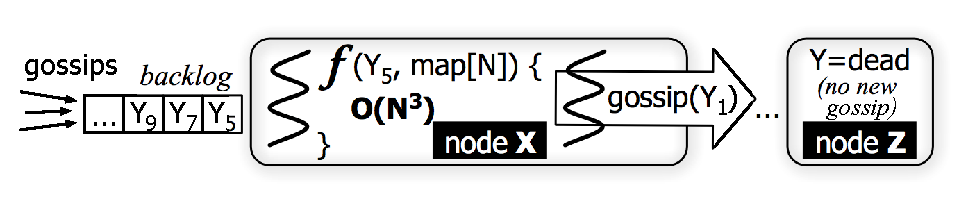
\includegraphics[height=0.8in]{F/cass1.eps}
%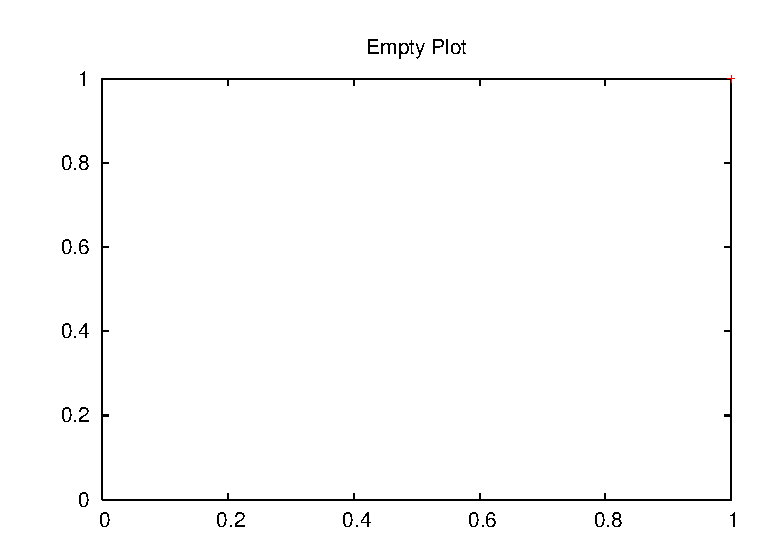
\includegraphics[height=0.6in]{F/empty.eps}
}
\vminfive
\mycaption{fig-cass1}{The problem of
gossip-based failure detection in Cassandra}{}
\vminfive
\end{figure}



We now describe in detail a scalability bug in Cassandra, which we use as a
sample bug.
%
Our journey in understanding scalability bugs began when we observed repeated
``flapping'' problems in large-scale Cassandra deployments (\ie, hundreds of
nodes).
%
Flapping is a cluster instability problem where node's up/down status
continuously flaps.  A ``flap'' is when a node X marks a peer node Y as down
(and soon marks Y as alive again).
%
We rigorously study a series of Cassandra bugs below that surfaced as the code
evolved.

%
%The bug surfaced on a cluster with hundreds of nodes and led to
%``\textit{\textbf{flapping}}'' nodes, a condition where node up/down status
%continuously changes;  tens of thousands of flaps\footnote{A ``\textbf{flap}''
%is when a node X marks a peer node Y as down.}  were observed.

To understand this bug, we need to understand the following protocols.

\begin{enumerate}

\item {\bf Bootstrap:} Each node first creates partition keys (\eg, 32 random
numbers) and gossips this information to peer nodes.
 
\item {\bf Gossip broadcast:} {\em Every second}, each node gossips to one
random node about a list of nodes and partitions it knows (including itself)
and their {\em version} numbers.  Each node also increments its version number
(``I'm still alive'') before gossiping.
 
\item {\bf Gossip processing:} The receiving node then finds any state
(metadata) differences between the two nodes to synchronize their views of the
ring.  Eventually, all nodes know about each other.
 
\item {\bf Failure detection:} {\em Every second}, a failure detection daemon
runs \cite{Lakshman+09-Cassandra}.  Put simply, if a node X has not received a
new gossip about Y {\em from anyone} (Y's version has not changed after some
period of time), X will declare Y dead (a flap).  When X receives a new gossip
about Y, it marks Y alive.

\end{enumerate}

% about the bug
There are two factors that induce the bug. The first is the {\em long latency
of scale-dependent state-update gossip processing during bootstrapping} (``f''
in Figure \ref{fig-cass1}).  While gossip processing is usually fast in a
stable cluster, it is expensive during bootstrapping as the gossips carry many
new state changes about the ring; the state-update processing time is
scale-dependent (\ie, greater than $O(N^3)$); the larger the cluster ($N$), the
larger the ring map, the longer the processing time is.
%
This long latency is caused by {\bf (1)} state-update checkpoint to on-disk
database and {\bf (2)} multi-map cloning and updates.
%
The first one is needed for fast fault tolerance; after a node crashes, it can
reboot fast as it knows the latest view of the ring.
%
The second one is preferred for simplicity; Cassandra clones its \ts{MultiMap}
ring table and applies changes one by one to alleviate long write locks.
%
% in order to prevent a long write lock on the ring table which can block other
% user-facing protocols.

% long
The second factor is the {\em single threaded} implementation of gossip
processing. As shown in Figure \ref{fig-cass1},  this inability to process
multiple gossips/state updates concurrently (for the sake of preventing
concurrency bugs) creates a {\em backlog} of new gossips.  For example, in {\em
every second}, Y tells someone it's alive with increasing version number (\eg,
Y$_7$), but the receiving nodes are still busy processing state changes and
only forward Y's old version number (\eg, Y$_1$).  As Y's new gossip is not
propagated on time,  other nodes (\eg, Z) will mark Y as dead.  This happens to
all nodes, not just Y.

% \ca{3831} -------------------------------------------------
The journey starts with Bug \#\ca{3831} \cite{CA-Two}, when a node D is
decommissioned from a cluster ring, D initiates a gossip telling that all other
nodes must rebalance the ring's key-ranges.  This scale-dependent ``pending
key-range calculation'' is CPU intensive with
%
% $O((n^2)log(n))$   % OLD
$O(MN^3log^3(N))$  % Tanakorn
%
complexity; $M$~is the list of key-range changes in the gossip message.  This
in turn leaves many gossips not propagated on time, creating flapping symptoms
that only appear at scale (at 200+ nodes; \sec\ref{sec-eval}). The developers
then optimized the code to
%
% $O(nlog(n))$  % OLD
$O(MN^2log^2(N))$ complexity.



% \ca{3881} -------------------------------------------------
Soon afterwards (Bug \#\ca{3881} \cite{CA-Tri}), Cassandra added the concept of
virtual partitions/nodes (\eg, $P$$=$$256$ per physical node).  As an
implication, the fix above did not scale as ``$N$'' becomes $N$$\times$$P$.
%
The bug was fixed with a complete redesign of the pending key-range
calculation, making it
% $O(log(N))$ OLD
$O(MNPlog^2(NP))$.

% \ca{5456} -------------------------------------------------
About a year later (\ca{5456} \cite{CA-Four}), Cassandra code employs
multi-threading between the pending key-range calculation and the gossip
processing with a coarse-grained lock to protect sharing of the ring
table.  Unbeknownst to the developers, at scale, the key-range calculation
can acquire the lock for a long time, causing flapping to reappear again.
The fix clones the ring table for the key-range calculation, to release the
lock early.



% \ca{6127} -------------------------------------------------
Later on (\ca{6127} \cite{CA-One}), a similar bug reappeared.  In the above
cases, the problems appeared when the cluster grows/shrinks gradually.
However, if customers bootstrap a large cluster (\eg, 500+ nodes) from
scratch (\ie, all nodes do not know each other, with no established
key ranges),
%
the execution traverses a different code path that
performs a fresh ring-table/key-range construction with
$O(MN^2)$ % KORN
complexity.

% \tl{and there is no existing data stored in   the cluster}), 
% \tl{the offending function becomes the keyrange construction} 
%
% keyrange calculation which clones the ring table (a
% \ts{MultiMap}) becomes very expensive.  
%
% Including the cloning $O(N*P)$, we observed an 
% $O(N^3)$  $O(MN^2)$ % KORN complexity.

% ...............
The story continues on (\ca{6345}, \ca{6409}, \etc).  Fast forward today,
Cassandra developers recently started a new umbrella ticket for discussing
``Gossip 2.0,''  supposedly scalable to 1000+
nodes \cite{Gossip20, Gossip20Mail}.
% ---- 
Similar to Cassandra, other large-scale systems are prone to the same
problem.  So far, we have collected and analyzed \totCass Cassandra, \totCouch
Couchbase, \totHadoop Hadoop, \totHBase HBase, \totHDFS HDFS, \totRiak
Riak, and \totVold Voldemort scalability bugs, all caused user-visible
impacts.
%
This manual mining was arduous because there is no searchable jargon for
``scalability bugs''; we might have missed other bugs.
%

